\documentclass[12pt,a4paper, fleqn]{article}

\usepackage[utf8]{inputenc}
\usepackage[french]{babel}
\usepackage{tikz}
\usepackage[T1]{fontenc}
\usepackage{amsmath}																				% les maths
\usepackage{amsfonts}
\usepackage{amssymb}
\usepackage{fourier}																					% symboles intégral propre
\usepackage{graphicx}
\usepackage[left=2cm,right=2cm,top=2cm,bottom=2cm]{geometry}	% les marges
\usepackage{multicol}																					% pour écrire sur plusieurs colones
\usepackage[thinspace,thinqspace,amssymb]{SIunits}							% écriture des nombres et unités
\usepackage{setspace}																				% set space between lines
\usepackage{array}																						% stretch array lines
\usepackage[hyphens]{url}
\usepackage[breaklinks]{hyperref}															% clickable links
%\usepackage[hyphenbreaks]{breakurl}														% for long urls
\usepackage{chemfig}																					% pour les formules chimiques
\usepackage{pdflscape}

\hypersetup{
    colorlinks=true,
    linkcolor=red_f,
    citecolor=bleu_f,
    filecolor=green_f,
    urlcolor=bleu_f
}

\usepackage{xcolor}																			% colors
\usepackage[framemethod=tikz]{mdframed}									% fancy environments

%%%%%%%%%% graphic charter

\renewcommand{\familydefault}{\sfdefault}												% sans serif font

%%%%% HEADER
%\pagestyle{fancy}
%\lhead{\textcolor{gray_f}{Physique-Chimie\\R. METZDORFF}}
%\chead{\textcolor{gray_f}{Lycée Suzanne Valadon}}
%\rhead{\textcolor{gray_f}{2020-2021}}
%\renewcommand{\headrulewidth}{0.4pt}
%\let\HeadRule\headrule
%\renewcommand\headrule{\color{gray_f}\HeadRule}

%%%%% COLORS
\definecolor{gray_f}{RGB}{68,84,106}
\definecolor{gray_c}{RGB}{214,220,229}
\definecolor{gray_cc}{RGB}{245,245,245}
\definecolor{bleu_f}{RGB}{91,155,213}
\definecolor{bleu_c}{RGB}{222,235,247}
\definecolor{red_f}{RGB}{204,0,0}
\definecolor{red_c}{RGB}{245,204,204}
\definecolor{orange_f}{RGB}{237,125,49}
\definecolor{orange_c}{RGB}{251,229,214}
\definecolor{green_f}{RGB}{112,173,71}
\definecolor{green_c}{RGB}{226,240,217}
\definecolor{yellow_f}{RGB}{255,192,0}
\definecolor{yellow_c}{RGB}{255,242,204}
\definecolor{code_keyword}{RGB}{23,23,139}										% colors for pyhton code
\definecolor{code_comment}{RGB}{50,137,21}
\definecolor{code_string}{RGB}{139,139,25}
\definecolor{red_unilim}{RGB}{166,41,41}
\definecolor{gray_unilim}{RGB}{78,87,94}
\definecolor{orange_unilim}{RGB}{209,98,40}

%%%%% NEW ENVIRONMENTS

%%% header
\mdfdefinestyle{s_head}{%
	linecolor=red_unilim!,
	outerlinewidth=3pt,%
	frametitlerule=false,
	topline=false,
	bottomline=false,
	rightline=false,
	leftline=false,
	backgroundcolor=red_unilim,
	innertopmargin=8pt,
	roundcorner=0pt,
	nobreak=true,
	fontcolor=white
}
\newmdenv[style=s_head]{header_env}
\newenvironment{header}
{%\stepcounter{exa}%
	\addcontentsline{ldf}{figure}{0}%
	\begin{header_env}\qquad\Large\bf}
	{\end{header_env}}

%%%%% New command

\newcommand{\app}{\colorbox{bleu_c}{\textcolor{bleu_f}{APP}}}
\newcommand{\rea}{\colorbox{yellow_c}{\textcolor{yellow_f}{REA}}}
\newcommand{\anarai}{\colorbox{green_c}{\textcolor{green_f}{ANA-RAI}}}
\newcommand{\val}{\colorbox{orange_c}{\textcolor{orange_f}{VAL}}}
\newcommand{\com}{\colorbox{red_c}{\textcolor{red_f}{COM}}}
\newcommand{\auto}{\colorbox{white}{\textcolor{black}{AUTO}}}
\newcommand{\rco}{\colorbox{gray_c}{\textcolor{gray_f}{RCO}}}
\newcommand{\seconde}{2\textsuperscript{nde}}

\bibliographystyle{custom-bib/thesis}
\usepackage{bibentry}
\usepackage{pdfpages}

\title{L'expérience de Benjamin Franklin... Et Rayleigh, Pockels, Devaux, et Langmuir}
\author{Rémi Metzdorff}
\date{\today}

\onehalfspacing

\begin{document}

%\maketitle

\begin{header}
\begin{minipage}{0.55\textwidth}
Rapport de stage (S4)
\end{minipage}
\begin{minipage}{0.38\textwidth}
\href{https://www.unilim.fr/}{
\includegraphics[scale=1]{logo.png}}
\end{minipage}
\end{header}

\vspace{30pt}
\begin{spacing}{1.2}
{\bf
\begin{Large}
\noindent
\textcolor{gray_unilim}{INSPE Académie de Limoges}
\end{Large}

\begin{large}
\noindent
\textcolor{gray_unilim}{Métiers de l'enseignement, de l'éducation et de la formation}

\noindent
\textcolor{gray_unilim}{Master MEEF Second degré}

\noindent
\textcolor{gray_unilim}{Professeur de Physique et de Chimie}

\noindent
\textcolor{gray_unilim}{Accompagnement à la mise en situation professionnelle}

\end{large}
}

\vspace{20pt}

\noindent
\textcolor{gray_unilim}{2020--2021}

\vspace{40pt}
\begin{large}
\bf
\noindent
\textcolor{gray_unilim}{Analyse d'une séance autour de la mesure de la taille d'une molécule d'huile d'après l'expérience de Franklin}

\vspace{150pt}
\noindent
\textcolor{gray_unilim}{Rémi Metzdorff}

\noindent
\textcolor{gray_unilim}{Lycée Suzanne Valadon}
\end{large}
\end{spacing}

\vfill

\hfill

\includegraphics[scale=1]{logo_bottom.png}

\thispagestyle{empty}

\newpage

\tableofcontents
\newpage

\section*{Introduction}
\addcontentsline{toc}{section}{Introduction}

Ce rapport présente le déroulement et l'analyse a posteriori de la séance réalisée le 7 décembre 2020 avec le groupe 1 de la classe de seconde 1, entre 14h50 et 16h15, à l'occasion de la première visite conjointe de mon tuteur établissement (M. Laurent Astier) et de ma tutrice INSPE (Mme Claire Maumy).
Il est la suite du dossier constitué au S3 où la séance est présentée en détail.
On en rappelle ici succinctement les grandes lignes.

L'objectif de la séance est de déterminer la taille d'une molécule de trioléine en exploitant l'expérience historique de Benjamin Franklin qui est surpris par l'ampleur de la surface recouverte par un film d'huile après en avoir versé une cuillère à café à la surface d'un étang.
Les élèves doivent pour cela :
\begin{itemize}
\item[•] déterminer le volume d'une cuillère à café ;
\item[•] déterminer la surface du film d'huile à la fin de l'expérience ;
\item[•] en déduire l'épaisseur du film d'huile ;
\item[•] faire le lien avec la taille d'une molécule d'huile pour conclure et répondre au problème.
\end{itemize}
Le sujet élève est en annexe (Ann.~\ref{ann:sujet}).

\section{Déroulement de la séance}

L'activité utilisée pendant la séance a été proposée à deux autres groupes avant celui-ci.
Le début de la séance se déroule donc sans surprise majeure et suit le déroulement prévu même si certaines étapes sont très perfectibles comme on le verra.
Il est difficile de relater précisément le déroulement de la suite de la séance puisqu'il s'agit principalement  d'interactions avec les groupes, en essayant de comprendre au mieux les difficultés rencontrées par chaque groupe pour les aider à avancer, en leur consacrant un temps suffisant tout en restant disponible pour le reste de la classe.

Les moments clés de la séance sont identifiés ci-dessous, en se basant notamment sur les observations du rapport de séance du tuteur établissement rédigé pour l'occasion.
Les compétences mentionnées ci-dessous font référence aux compétences évaluées pendant la séance (ann.~\ref{ann:cptces}).
L'évaluation globale de la séance repose sur les compétences évaluées pendant la séance (Ann.~\ref{ann:suivi}) et sur le compte-rendu des groupes.
Elle est résumée dans le tableau disponible en annexe (Ann.~\ref{ann:eval}).

\paragraph{14h55 : Accueil}
\begin{itemize}
\item[•] entrée en classe avec désinfection des mains ;
\item[•] les élèves se répartissent en binôme ;
\item[•] appel : sept élèves manquent à l'appel ;
\item[•] présentation de la séance et contextualisation.
\end{itemize}

\paragraph{15h00 : Retardataires}
\begin{itemize}
\item[•] trois élèves arrivent en retard : ils s'installent rapidement pour former un binôme et un monôme.
\end{itemize}

\paragraph{15h01 : Lancement de l'activité}
\begin{itemize}
\item[•] consignes ;
\item[•] distribution des sujets ;
\item[•] la question centrale est écrite au tableau ainsi que l'aide à la rédaction du compte-rendu.
\item[•] préparation de la grille de notation (Ann.~\ref{ann:suivi}) pendant que les élèves découvrent le sujet.
\end{itemize}

\paragraph{$\sim$ 15h15 -- 15h20 Hypothèse}
\begin{itemize}
\item[•] la plupart des groupes bénéficient du coup de pouce 5 (Ann.~\ref{ann:aides}) pour formuler leur hypothèse ;
\item[•] les premiers élèves commencent à demander la vérification de leur hypothèse ;
\item[•] plusieurs groupes n'appellent pas et je vais les voir pour qu'ils n'y passent pas un temps déraisonnable.
\end{itemize}

\paragraph{$\sim$ 15h20 -- 15h45 Évaluation d'une première compétence}
\begin{itemize}
\item[•] suivant les groupes, c'est la compétence \anarai{}, \app{} ou \rea{} qui est évaluée en premier ;
\item[•] deux groupes sur sept ont pu proposer un début de protocole pour répondre au problème.
\item[•] les autres groupes sont débloqués par le coup de pource les invitant à mesurer le volume d'une cuillère à café.
\end{itemize}

\paragraph{$\sim$ 15h30 -- 16h05 Évaluation d'une deuxième compétence}
\begin{itemize}
\item[•] suivant les groupes, c'est la compétence \anarai{} ou \rea{} qui est évaluée ensuite ;
\item[•] vient ensuite pour la plupart des groupe de la surface du film d'huile : le coup de pouce 3 (Ann.~\ref{ann:aides}) est parfois utile.
\end{itemize}

\paragraph{$\sim$ 15h50 -- 16h10 Épaisseur du film d'huile}
\begin{itemize}
\item[•] le coup de pouce 4 (Ann.~\ref{ann:aides}) est ici nécessaire à tous les groupes pour avancer vers la conclusion.
\end{itemize}

\paragraph{$\sim$ 16h10 -- 16h15 Conclusion et fin de séance}
\begin{itemize}
\item[•] évaluation de la compétence \val{} pour deux groupes ;
\item[•] ramassage des compte-rendus ;
\item[•] fin de séance
\end{itemize}

\section{Analyse a posteriori}

Dans cette section, le déroulement réel de la séance est comparé au déroulement prévu dans la section 2.5 du précédent rapport.
Quand il y a lieu, des propositions pour l'amélioration de la séance sont envisagées.

\subsection{Sur le déroulement de la séance}

Pour cette séance, la consigne auraient pu être passée avec plus de clarté et en attendant que tous les élèves soient attentifs.
Ils se sont toutefois bien mis au travail car à ce stade de l'année, ils sont familiers avec la consigne \og Un CR chacun chacune, le prof en ramasse un par groupe en fin de séance \fg{}.
Le repère temporel de 15 min pour l'hypothèse n'a cependant pas été convenablement perçu et il a fallu passer parmi les groupes pour leur demander leur hypothèse avant qu'ils ne passent à la suite.
À ce stade de l'année, les appels profs n'étaient pas suffisamment formalisés.
Ils auraient pu apparaitre par exemple sur le sujet (Ann.~\ref{ann:sujet}) dans l'aide à la rédaction et/ou au tableau.
La consigne de temps aurait pu être inscrite au tableau.
En plus de ces éléments, il aurait été préférable de s'assurer que les élèves étaient réellement attentifs au moment du passage de la consigne, en appuyant davantage sur la première étape (l'hypothèse) et sa durée.

La gestion des élèves retardataires auraient pu être améliorée.
Inclure ces élèves dans des groupes présents depuis le début de la séance aurait peut-être permis de les mettre plus rapidement en activité.
Cela aurait aussi évité qu'un élève se retrouve seul ce qui a été un frein pour lui concernant cette séance.
Il aurait aussi fallu leur consacrer un temps plus important pour s'assurer qu'ils aient bien compris l'objectif de la séance.

Finalement, le choix de former des binômes, particulièrement pour cette séance est discutable.
Afin d'encourager davantage le conflit socio-cognitif, il aurait été intéressant de former des groupes plus importants : selon \cite{Courtillot2006}, le nombre idéal d'élèves dans un groupe est de quatre pour que l'apport de ce débat soit optimal.
\footnote{Après cette séance, la même activité a été proposée à un dernier groupe en imposant cette fois la formation de trinômes et leur composition.
La moitié des groupes sont parvenus à conclure l'activité pendant la séance (contre un seul ici) et les compte-rendus étaient globalement meilleurs que pour cette séance.}
Sur cette activité, un travail en îlots est sans doute très bénéfique aux élèves.
Dans ce cas une évaluation individuelle de la contribution des élèves semble très difficile à réaliser, mais il y a aussi d'autres occasions pour cela.

Pour cette séance, seul un groupe est parvenu à la conclusion de l'activité pendant la séance.
Pour les autres, la conclusion est arrivée à la séance suivante, alors que la présentation d'un court travail de recherche bibliographique permettait de revenir sur le sujet.
En cela l'objectif d'ancrer l'ordre de grandeur des entités microscopiques constituant la matière qui rejoint la capacité exigible du programme \og Citer l'ordre de grandeur de la valeur de la taille d'un atome \fg{} n'est pas vraiment atteint.
En revanche, le travail sur les compétences de la démarche scientifique et la démarche de résolution de problème justifie bien a posteriori l'activité proposée.
Comme l'a montré la séance suivante, l'objectif principal demeure atteignable par un plus grand nombre d'élèves en modifiant certains éléments.

\subsection{À propos des conceptions initiales}

Parmi les conceptions initiales identifiées dans le premier rapport, l'une est apparue lors de la formulation de l'hypothèse chez un groupe d'élèves.
En observant les gouttelettes d'huile qui tombent quand on la fait couler, ils pensaient que les molécules étaient ces gouttelettes : \og les mêmes que celles dans une vinaigrette ou à la surface d'un bouillon \fg{}.
On peut rapprocher ces confusions de celles identifiées par \cite{Bain1985} concernant une absence de structure microscopique de la matière, ou plus certainement de l'idée de molécules macroscopiques évoquée dans \cite{Griffiths1992}.
Les élèves proposaient donc une taille pour la molécule d'huile de l'ordre du millimètre.
Le coup de pouce 5 (Ann.~\ref{ann:aides}) a permis de les amener rapidement à une hypothèse plus raisonnable.
Au début de l'activité, il est possible que la difficulté à imaginer un protocole permettant de mesurer une molécule réellement microscopique les ait induit en erreur : ils souhaitaient en effet mesurer ces gouttes à l'aide d'une règle, outils adapté pour mesurer des longueurs jusqu'au millimètre.

Les autres conceptions initiales ne sont pas ressorties et la plupart des élèves semblent s'être bien appropriés le concept de molécule à ce stade de leur scolarité.

\subsection{À propos des prérequis}

Bien que le sujet puisse être déstabilisant, les élèves se sont plutôt bien raccrochés à l'aide à la rédaction du compte-rendu qu'ils avaient déjà utilisée dans d'autres activités.
Les différentes étapes de la démarche ont été convenablement respectées.

Pour la grande majorité des élèves, la discontinuité de la matière n'a pas posé de problème particulier.
Des confusions entre atome et molécule sont présentes mais la question : \og Avec quoi sont formées les molécules ? \fg{} suffit pour lever l'ambiguïté.

Le coup de pouce 5 (Ann.~\ref{ann:aides}) a bien aidé les élèves à proposer une hypothèse cohérente en début d'activité en réinvestissant le raisonnement mobilisé pour mesurer le personnage de la vidéo \href{https://youtu.be/oSCX78-8-q0}{A boy and his atom}.
Certains élèves ont compté tous les atomes de la molécule au lieu de ne considérer que les atomes de carbone des chaines carbonées, ce qui conduit à une surestimation de la taille de la molécule.
Cette \og erreur \fg{} était visible dans plusieurs compte-rendus mais je ne l'ai pas toujours remarquée pendant la séance.
Montrer un modèle moléculaire d'une partie de la molécule pourrait aider les élèves à se rendre compte de la forme de cette molécule et les aider à interpréter la représentation du coup de pouce.
L'ordre de grandeur trouvé par les élèves reste correct et n'a pas semblé perturber outre mesure le reste de l'activité.

La manipulation des puissances de dix, même si elle n'était pas encore maitrisée par tous, n'a pas été un obstacle majeur.

Finalement, pour ce qui est des compétences expérimentales :
\begin{itemize}
\item[•] mesurer un volume à l'aide d'une éprouvette graduée : pas de problème particulier ;
\item[•] mesurer des distances sur un schéma à l'aide d'une échelle de longueur : c'est un point que j'avais supposé comme prérequis mais qui ne l'est pas.
Cette étape a été beaucoup plus chronophage que prévu pour de nombreux groupes et aurait pu être mieux préparée.
On aurait pu proposer ici plusieurs sujets pour s'adapter davantage aux différents profils d'élèves et mettre en place une différenciation pédagogique supplémentaire (Sec.~\ref{sec:sujet}).
\item[•] on aurait pu rajouter : mesurer une masse à l'aide d'une balance pour les groupes ayant choisi de mesurer un volume en passant par la masse volumique.
Les groupes arrivent à leur fin même si parfois, la mesure se fait sans récipient, en versant l'eau contenue dans la cuillère directement sur le plateau de la balance.
\end{itemize}

\subsection{À propos du sujet}
\label{sec:sujet}

Pour cette activité, si les compétences mobilisées sont identifiées, les critères d'évaluation ne sont pas clairement énoncés dans le sujet.
Ce choix est discutable.
D'un côté l'évaluation n'est pas complètement transparente  ce qui va l'encontre des préconisations de la loi du 8 juillet 2013 \cite{Loi2013} : \og Les modalités de la notation des élèves doivent évoluer pour éviter une « notation-sanction » à faible valeur pédagogique et privilégier une évaluation positive, simple et lisible, valorisant les progrès, encourageant les initiatives et compréhensible par les familles \fg{}.
L'objectif n'est cependant pas ici de piéger les élèves, mais plutôt de leur laisser la possibilité d'aborder le problème de différentes manières, en les incitant le moins possible à suivre un chemin de résolution particulier.
Ceci a pu contribuer je pense à l'émergence de pistes de résolution que je n'avais pas envisagées initialement.
Même si les élèves doivent nécessairement passer par certaines étapes qui leur donnent les résultats utiles à la conclusion de l'activité, on a ainsi pu assister à différents raisonnements : 
\begin{itemize}
\item[•] mesure du volume de la cuillère à café avant la mesure de l'aire du film d'huile et inversement ;
\item[•] mesure du volume directe (éprouvette graduée) ou en passant par la masse volumique ;
\item[•] mesure de la surface du film d'huile en mesurant l'aire du cercle ou en mesurant la surface de l'étang (le texte stipule qu'un quart de l'étang est recouvert par l'huile).
\end{itemize}

Lors de la première étape, quelques élèves se sont appuyés sur l'aide à la conversion donnée dans le sujet : $\unit{1}{mL} = \unit{1 \times 10^{-6}}{m^3} $ et ont proposé une hypothèse similaire à \og une molécule d'huile a une taille de \unit{1}{mL} \fg{}.
Ici, leur préciser qu'on attend une longueur a souvent permis de les orienter vers une hypothèse plus raisonnable.
Changer le titre de la section \og Donnée \fg{} du sujet en \og Aide à la conversion \fg{} pourrait peut-être éviter la confusion.

Comme le texte historique le suggérait (\og ce quart de l'étang \fg{}), la mesure de la surface du film d'huile peut passer par la mesure de la surface totale de l'étang.
On peut alors proposer un schéma différent aux élèves les plus en difficulté, où la longueur d'un côté de l'étang serait directement écrite, plutôt que de donner l'échelle à côté du schéma.
La compétence \rea{} est toujours mobilisée mais c'est peut-être alors la compétence \app{} qu'il est pertinent d'évaluer.
Ceci permettrait d'avancer plus rapidement vers la conclusion de l'activité si cela reste l'objectif privilégié de la séance.
Il s'agit ici de contourner une compétence périphérique pour atteindre le cœur de cible avec ces élèves \cite{Benoit2012}.

De la même façon, le coup de pouce 4 (Ann.~\ref{ann:aides}) pourrait être exprimé directement avec la formule :
\[e = \frac{V}{S}, \]
pour orienter directement les élèves les moins à l'aise avec les manipulations mathématiques vers le calcul à effectuer.

Cette aide est restée obscure pour plusieurs élèves qui n'y voyaient aucun lien avec l'activité.
Non prévue initialement, la proposition de leur faire dessiner le film d'huile en 3D les a bien aidés à faire le lien.

Finalement, pour aider les élèves à conclure en faisant le lien entre l'épaisseur du film et la taille d'une molécule, une poignée de pois cassés était prévue pour reproduire à grande échelle la manipulation.
Cette aide n'a pas réellement pu être testée par manque de temps mais il apparait que la plupart des élèves concluent en utilisant le résultat de l'épaisseur du film d'huile pour répondre au problème mais sans que le lien ne soit explicite.
À la séance suivante, ce lien a semblé plus clair pour beaucoup en s'appuyant sur le schéma de la Fig.~\ref{fig:exp}.

\begin{figure}
\center

\includegraphics[scale=.25]{experience.png}
\caption{Représentation de l'huile formant un film monomoléculaire à la surface de l'étang.}
\label{fig:exp}
\end{figure}

Les coups de pouce et aides apportés pendant la séance restent pertinents je crois, puisqu'ils permettent de s'adapter aux différentes démarches mises en place par les élèves.
Certains élèves ayant choisi de commencer par la mesure de la surface du film d'huile ont ainsi pu avancer en autonomie plus librement.
Lors des premières séances, l'aide visant à orienter les élèves vers la mesure du volume de la cuillère à café était fournie à l'ensemble de la classe : cela n'avait pas de sens pour ceux qui choisissent de commencer par mesurer la surface du film.

\section*{Conclusion}
\addcontentsline{toc}{section}{Conclusion}

La mise en place des modifications évoquées tout au long de ce rapport pourrait permettre à un plus grand nombre d'élèves de conclure correctement l'activité.
Bien que n'étant pas directement suggérée par les programmes de seconde, cette activité reposant sur l'exploitation de l'expérience historique de Benjamin Franklin me parait très pertinente pour les élèves, notamment au regard des compétences mobilisées pour avancer sur l'activité, et ce même si tous ne la terminent pas.
Une conclusion en classe entière permet d'aborder le point crucial de l'expérience qui n'est à l'évidence pas simple à identifier.
Preuve en est qu'il a fallu plusieurs dizaines d'années et de nombreux scientifiques pour découvrir les subtilités de cette expérience en apparence si banale et incongrue.

\newpage
\bibliography{biblio.bib}
\addcontentsline{toc}{section}{Références}

\newpage
\appendix

\section{Sujet élève}
\label{ann:sujet}

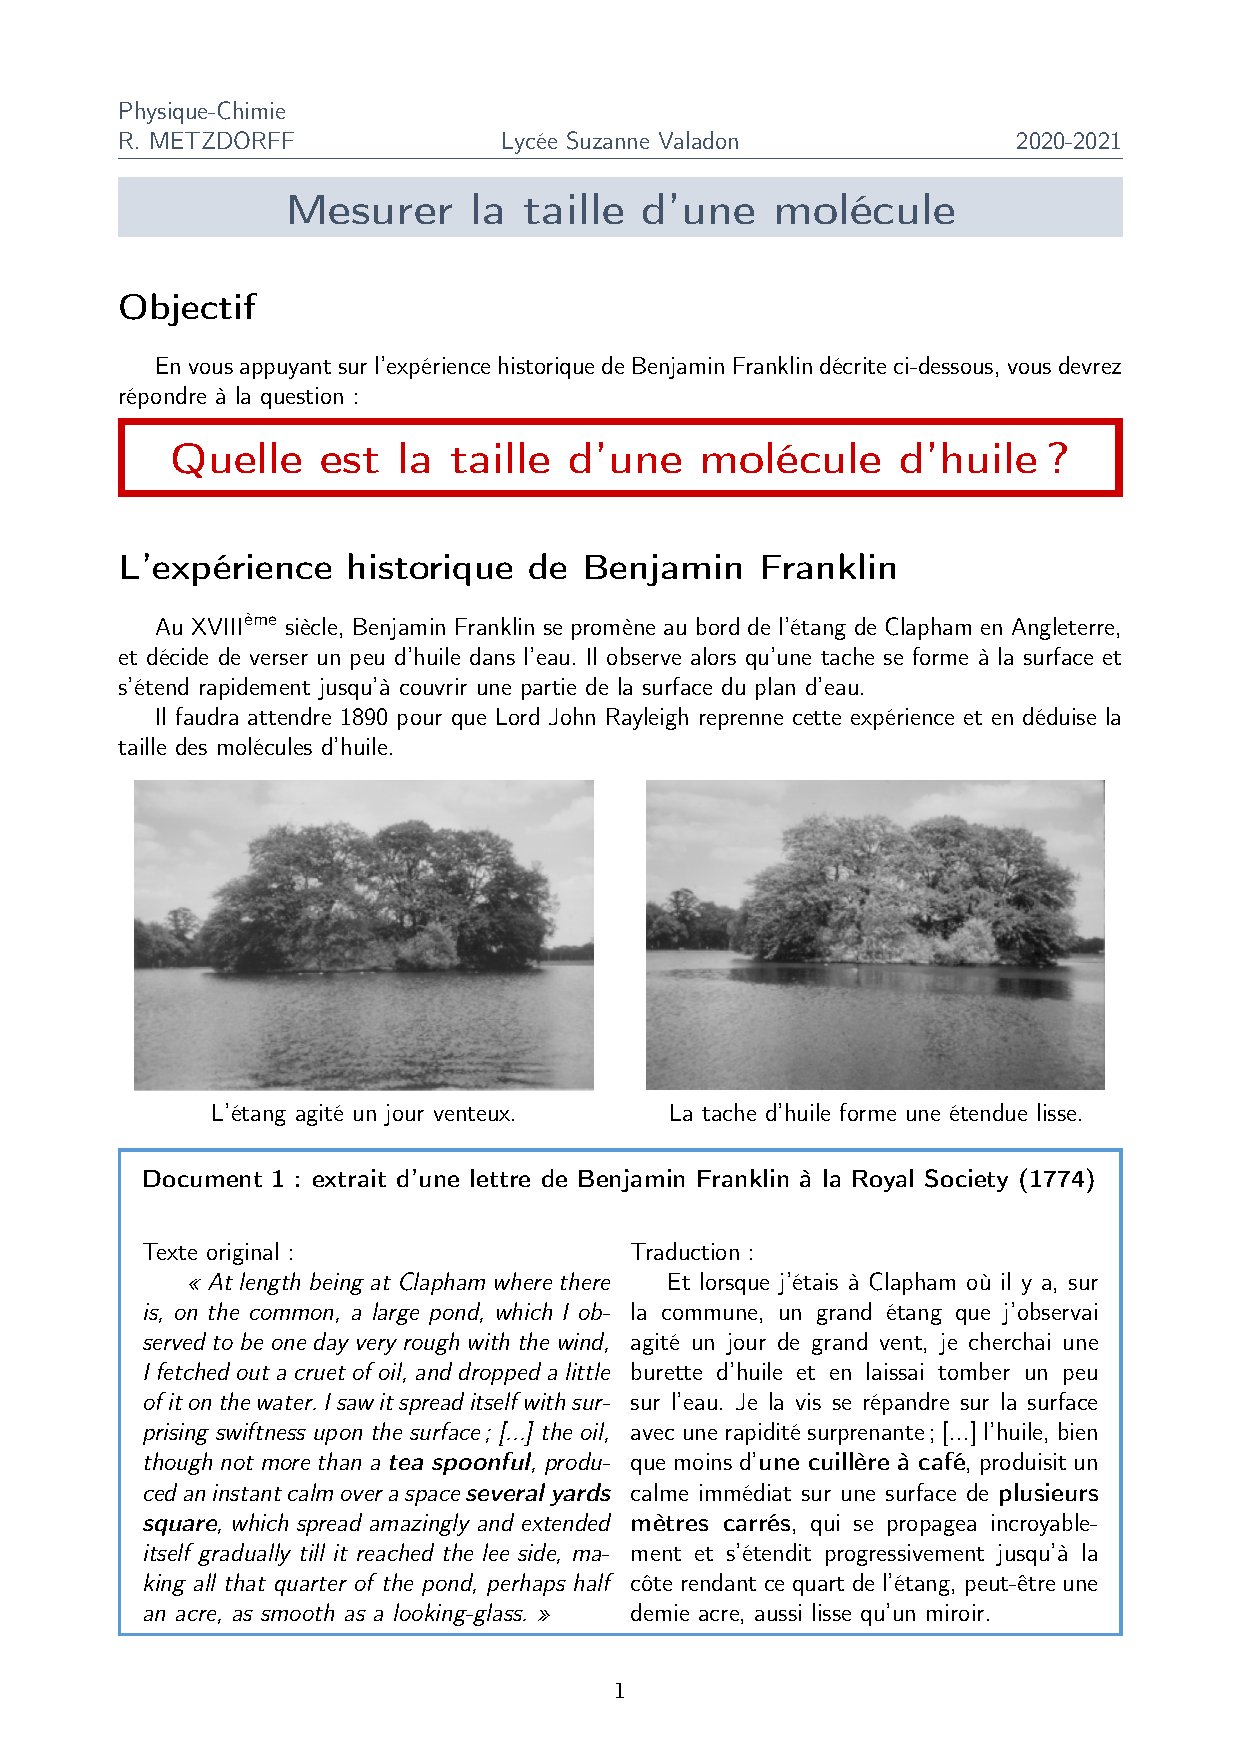
\includepdf[pages=-]{tp_franklin_v3.pdf}

\section{Aides}
\label{ann:aides}

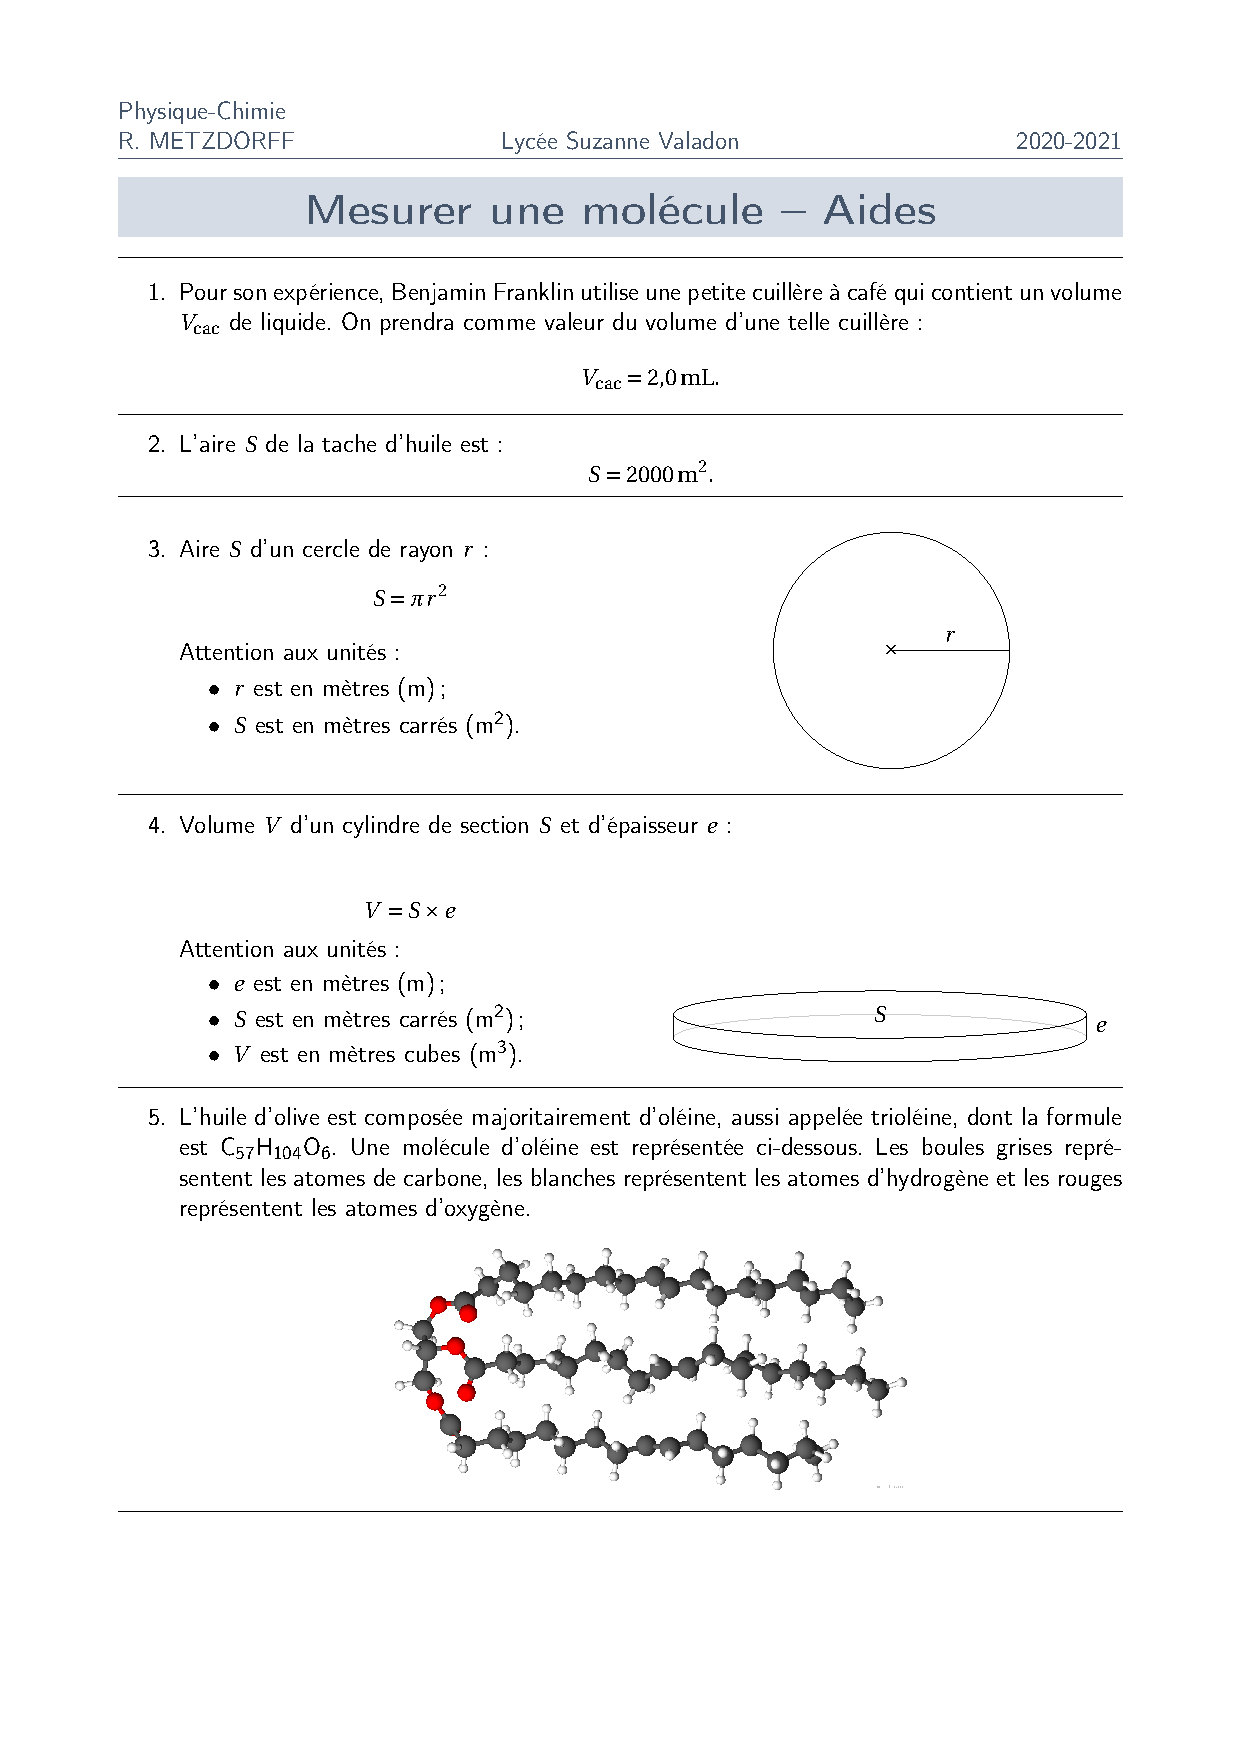
\includepdf[pages=-]{tp_franklin_aides.pdf}

\section{Proposition de correction}
\label{ann:corr}

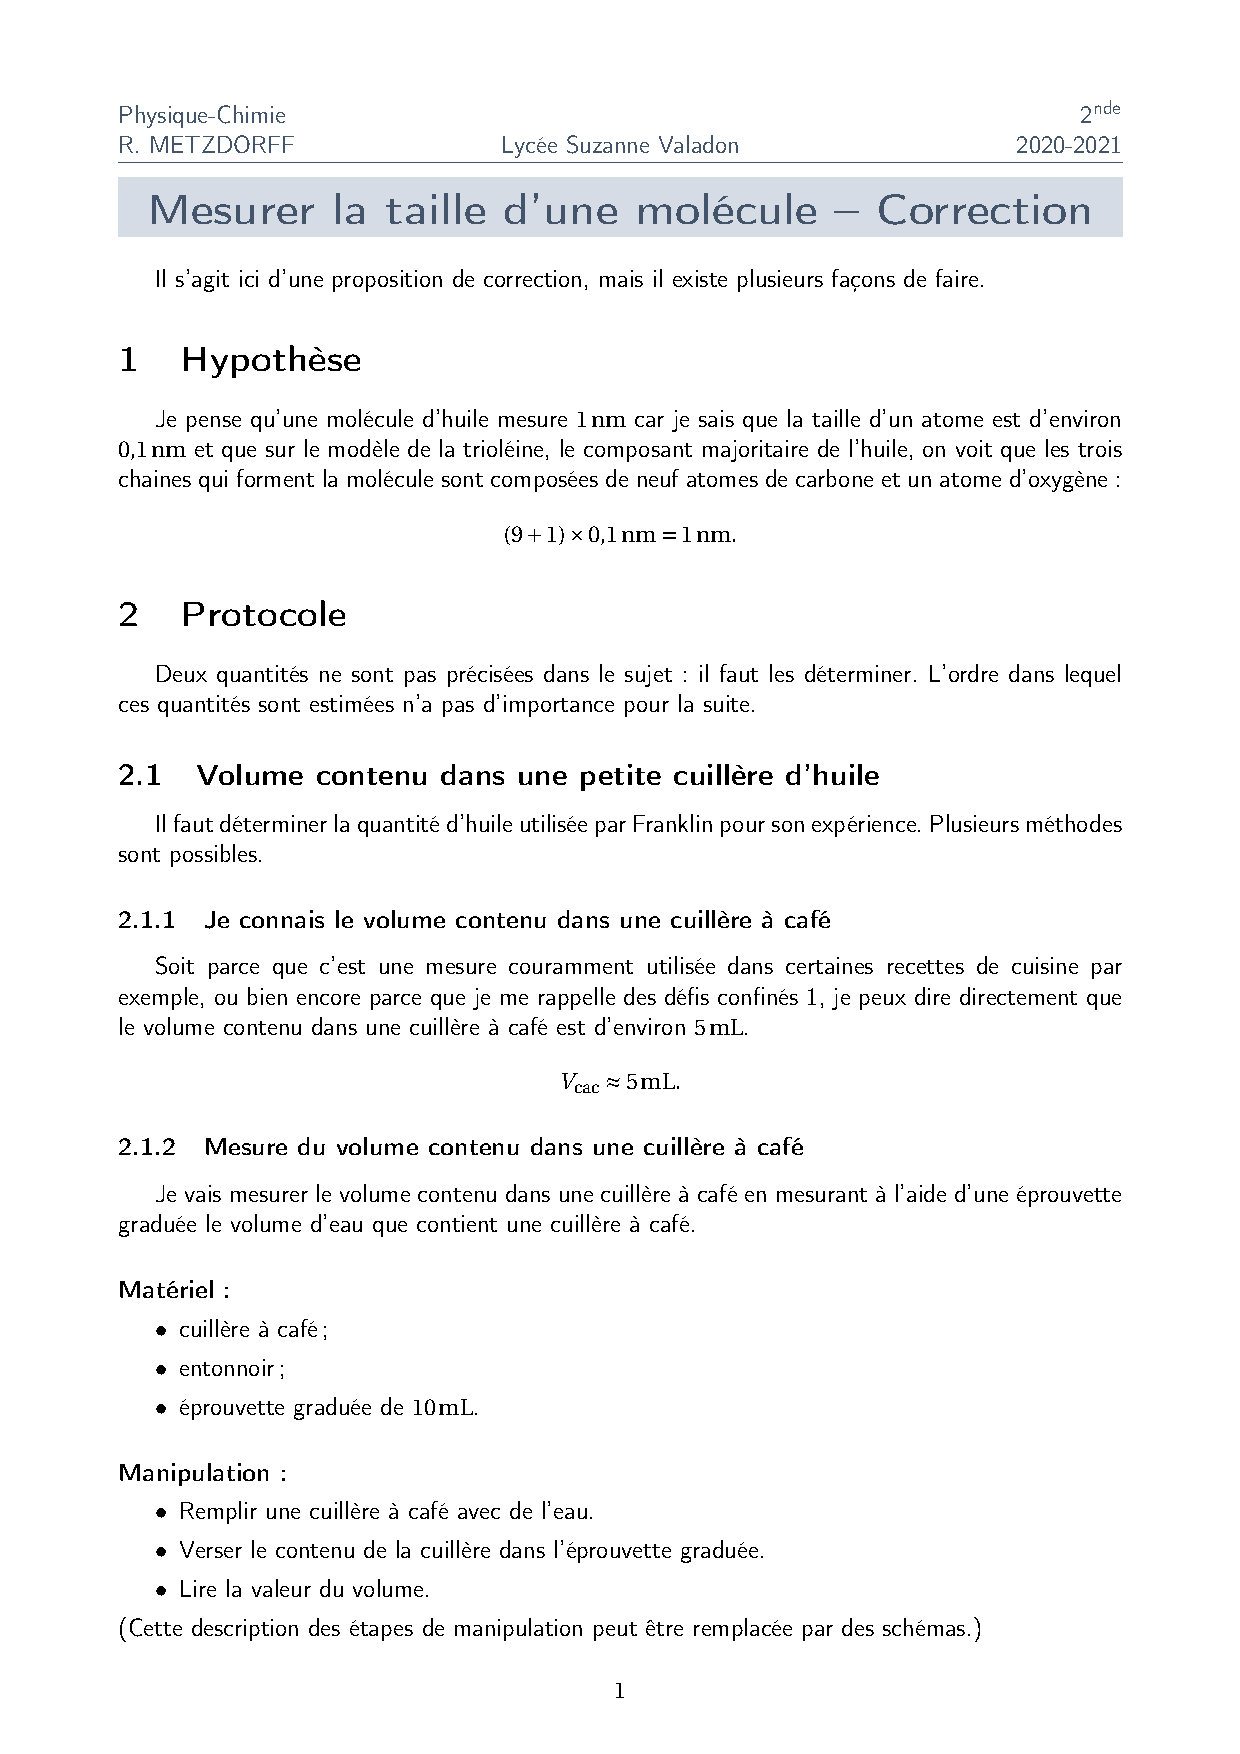
\includepdf[pages=-]{tp_franklin_corr.pdf}

\section{Compétences}
\label{ann:cptces}

Les tableaux ci-dessous identifient les compétences évaluées pendant la séance.
Le niveau de maîtrise de ces compétences est graduée selon quatre niveaux identifiables d'après l'aide apportée lors de la séance : A (bien maîtrisée), B (maîtrisée), C (insuffisamment maîtrisée) et D (non maîtrisée) (Tab.~\ref{tab:cptces_tp}).

\begin{table}[h]
\center
\begin{tabular}{l|l|c}
\textbf{Compétence} & \textbf{Aptitude} / Observable & \textbf{Niveau} \\
\hline \hline
\anarai 	& \textbf{Élaborer un protocole qui répond à la question} 	& \\
				& L'élève mesure le volume de 10 cac				 						& A+ \\
				& L'élève mesure le volume d'une cac 									& A \\
				& Aide : Avec quelle verrerie peut-on mesurer un volume ?	& B \\
				& Aide : Mesure le volume d'une cac d'huile avec une éprouvette & C \\
				& Aide : Une cac fait 5 mL 															& D \\
\hline
\rea			& \textbf{Faire des observations utiles à l'activité}					& \\
				& L'élève réalise la mesure de l'aire sur le schéma				& A \\
				& Aide : Dans la formule, quelles sont les valeurs connues ? & B \\
				& Aide : Mesure l'aire sur le schéma											& C \\
				& Aide : L'aire de la flaque est \unit{2000}{m\squared}			& D \\
\hline
\val			& \textbf{Avoir un regard critique sur ses résultats}				& \\
				& L'élève fait le lien avec son hypothèse									& A \\
				& Aide : Ça vous semble normal de trouver un chiffre aussi petit ? & B \\
				& Aide : Le professeur verse des haricots sur la table			& C \\
				& Aide : L'huile forme une couche haute comme une seule molécule & D \\
\end{tabular}
\caption{Observables utilisées pour l'évaluation du niveau de maîtrise des compétences travaillées lors de la séance.
\anarai{} : analyser-raisonner.
\rea{} : réaliser.
\val{} : valider.}
\label{tab:cptces_tp}
\end{table}

La compétence \app{} peut être mobilisée à la place de la compétence \anarai{} pour la détermination du volume de la cuillère à café, avec l'aptitude \og évaluer quantitativement les grandeurs physiques inconnues et non précisées \fg{}.


Le compte-rendu est aussi évalué sur la base des compétences mobilisées (Tab.~\ref{tab:cptces_cr}).

\begin{table}[h]
\center
\begin{tabular}{l|l}
\textbf{Compétence} & \textbf{Aptitude} \\
\hline \hline
\anarai 	& \textbf{Faire une hypothèse, la justifier} \\
\hline
\rea			& \textbf{Réaliser un schéma correspondant à la manipulation réalisée} \\
				& \textbf{Effectuer des procédures classiques (calculs, etc.)} \\
\hline
\val			& \textbf{Dire si mes résultats sont en accord avec ceux attendus} \\
 				& \textbf{Avoir un regard critique sur ses résultats} \\
\hline
\com		& \textbf{Rendre compte de façon écrite ou orale}
\end{tabular}
\caption{Compétences mobilisées et évaluées lors de la rédaction du compte-rendu.
\anarai{} : analyser-raisonner.
\rea{} : réaliser.
\val{} : valider.
\com{} : communiquer.}
\label{tab:cptces_cr}
\end{table}

\section{Fiche de suivi des élèves pendant la séance complétée}
\label{ann:suivi}

\begin{landscape}

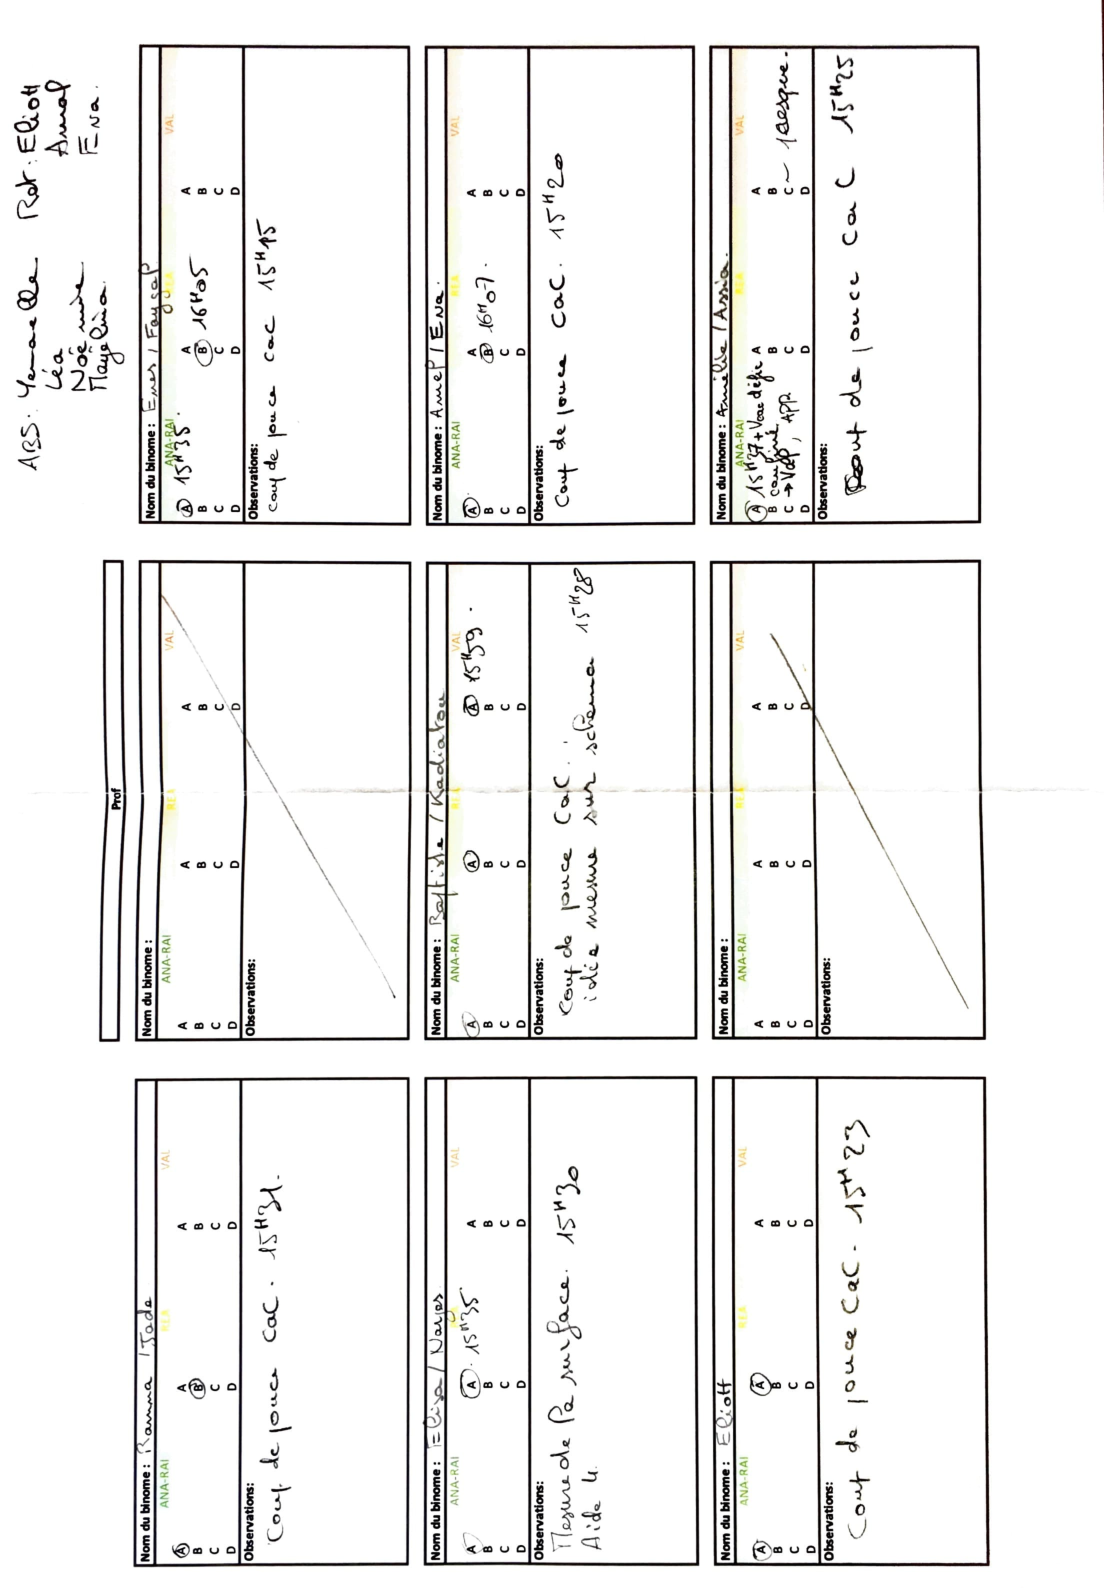
\includepdf[pages=-]{tp_franklin_prof_suivi.pdf}

\section{Évaluation de l'activité}
\label{ann:eval}
\vfill
\begin{table}[h]
\renewcommand\arraystretch{1.5}		% stretch table line height
\begin{center}
\begin{tabular}{|c|c|c|c|c|c|c|c|c|c|c|c|c|c|}
\hline
\textbf{Groupe} & \multicolumn{3}{c|}{\textbf{Séance}} & \multicolumn{4}{c|}{\textbf{Compte-rendu}} & \multicolumn{6}{c|}{\textbf{Total}} \\
\hline 
& \anarai & \rea & \val & \anarai & \rea &\val & \com & \app & \anarai & \rea & \val & \com & Note \\
\hline
& 5 & 5 & 3 & 1 & 3 & 2 & 1 & 0 & 6 & 8 & 5 & 1 & 20 \\
\hline\hline
\textbf{1} & A & B & & 1 & 2.5 & 0.5 & 1 & & 6 & 6.5 & 0.5 & 1 & 14 \\
\hline
\textbf{2} & A & A & & & 2.5 & 1.5 & 1 & & 5 & 7.5 & 1.5 & 1 & 15 \\
\hline
\textbf{3} & A & B & & 1 & 2 & 0.5 & 1 & & 6 & 6 & 0.5 & 1 & 13.5 \\
\hline
\textbf{4} & A & A & A & 1 & 2.5 & 1.5 & 1 & & 6 & 7.5 & 4.5 & 1 & 18 \\
\hline
\textbf{5} & A & A & & 0.5 & 0.5 & 0 & 1 & & 5.5 & 5.5 & 0 & 1 & 12 \\
\hline
\textbf{6} & A & B & & 1 & 1.5 & 0 & 1 & & 6 & 5.5 & 0 & 1 & 12.5  \\
\hline
\textbf{7} & A & B & C & 1 & 3 & 1 & 1 & & 6 & 7 & 2 & 1 & 16 \\
\hline
\end{tabular}
\end{center}
\caption{Bilan de l'évaluation de l'activité.}
\label{tab:eval}
\end{table}
\vfill
\end{landscape}

\end{document}